\chapter{ワークA：センサ回路設計}

\section{はじめに}
%% ワークAを理解した上で，目的として要約する
%%
%% （例文）
%%本課題では～を目的とし，～の実験を行った．
%% 実験を通じて～の結果を得た．
%% それらの結果より，～であることを明らかにする．

心拍に伴う血流量の変化を非侵襲的に検出する光電容積脈波計測法（Photoplethysmography: PPG）は，スマートウォッチやウェアラブル脈拍計などの生体情報モニタリング技術として広く普及している\cite{elgendi2019use, hertzman1938blood}．
光電容積脈波計測法では，生体組織に照射した光（赤外光や緑色光など）が動脈血中のヘモグロビンに吸収される特性を利用し，心臓の収縮・拡張に伴う毛細血管の容積変化を反射光または透過光の強度変化として光電変換素子により電気信号へと変換する．
しかしながら，生体組織の拍動によって得られる光電変換信号は極めて微小な交流成分（AC成分）であり，皮膚組織や静脈血による大きな直流オフセット成分（DC成分）に重畳している．
さらに，生体の体動や呼吸に伴う低周波の基線動揺（ドリフト），および室内照明や商用交流電源（50/60\,Hz）に起因する高周波ノイズが重畳するため，センサ出力をそのままマイコン等の処理系に入力しても正確な脈拍数を検出することは困難である．
したがって，所望の脈波信号周波数帯のみを通過させ，不要な直流成分や高周波ノイズを除去するとともに，信号処理系に適した電圧振幅まで信号を拡大するセンサ後段回路（バンドパスフィルタおよび増幅回路）の設計が不可欠である．

本課題（ワークA）では，反射型フォトリフレクタ（LBR-127HLD）を用いた脈拍検出回路，およびオペアンプ（LM358N）を用いたバンドパスフィルタ付き二段反転増幅回路を設計・実装し，その動作特性の評価を行うことを目的とした．
実験では，まず既知のテスト信号を生成可能な波形出力デバイス（ATOM Lite）を用い，設計した増幅回路の周波数特性および増幅率の動作検証を行った（ワークA-1）．
続いて，被験者の指先脈波をフォトリフレクタによって検出し，増幅・帯域制限された出力波形から心拍の周期および1分間あたりの脈拍数を計測した（ワークA-2）．
これらの実験を通じて，設計したアナログ増幅・フィルタ回路の伝達特性を評価するとともに，微弱な生体信号計測への適用可能性を検証する．


%-----------------------------------------------------------------------------------
\section{方法及び手順}
%% ワークAで設計・実装するものを理解した上で，方法や手順に落とし込んだ
%% 形で，客観的に記述する．報告書の基準は，この報告書の記述だけで，第
%% 三者が追試をし，同様の結果を得ることできることである．必要に応じて，
%% 図，表，式を用いて，曖昧な箇所や誤解を生じにくい説明が求められる．

\subsection{使用素子及び実験装置}

本実験で使用した電子部品一覧を表\ref{tab:circuit_components}に示す．また，回路作成および波形観測に使用した実験機器一覧を表\ref{tab:instruments}に示す．

\begin{table}[htbp]
  \caption{使用素子一覧}
  \centering
  \small
  \setlength{\tabcolsep}{5pt}
  \begin{tabular}{|l|c|r|l|}
    \hline
    部品名          & 数量 & \multicolumn{1}{c|}{仕様} & 素子変数                 \\
    \hline\hline
    炭素皮膜抵抗       & 1  & 330 $\Omega$            & $R_3$                \\
    \hline
    炭素皮膜抵抗       & 1  & 3.3 $\rm{k}\Omega$      & $R_4$                \\
    \hline
    炭素皮膜抵抗       & 4  & 33 $\rm{k}\Omega$       & $R_5, R_6, R_7, R_9$ \\
    \hline
    炭素皮膜抵抗       & 1  & 1 $\rm{M}\Omega$        & $R_2$                \\
    \hline
    炭素皮膜抵抗       & 3  & 100 $\rm{k}\Omega$      & $R_1, R_8, R_{10}$   \\
    \hline
    積層セラミックコンデンサ & 2  & 10 $\mu\rm{F}$          & $C_3, C_4$           \\
    \hline
    積層セラミックコンデンサ & 1  & 0.01 $\mu\rm{F}$        & $C_2$                \\
    \hline
    積層セラミックコンデンサ & 1  & 0.1 $\mu\rm{F}$         & $C_1$                \\
    \hline
    オペアンプ        & 1  & LM358N                  & ---                  \\
    \hline
    フォトリフレクタ     & 1  & LBR-127HLD              & ---                  \\
    \hline
  \end{tabular}
  \label{tab:circuit_components}
\end{table}

\begin{table}[htbp]
  \caption{使用実験機器一覧}
  \centering
  \small
  \setlength{\tabcolsep}{4pt}
  \begin{tabular}{|l|l|c|l|}
    \hline
    機器名      & 型式 / メーカー               & 数量 & 用途                \\
    \hline\hline
    オシロスコープ  & Tektronix TBS1000Cシリーズ  & 1台 & 入出力波形の観測および計測     \\
    \hline
    波形出力デバイス & ATOM Lite（M5Stack）      & 1台 & 評価用模擬信号（4種類）の発生   \\
    \hline
    直列抵抗     & 1 $\rm{M}\Omega$ 炭素皮膜抵抗 & 1本 & ATOM Lite信号減衰・保護用 \\
    \hline
    ブレッドボード  & 165401020E              & 1枚 & 回路実装用基板           \\
    \hline
    電源ユニット   & 5V安定化電源供給ユニット           & 1式 & 回路駆動用電源（5V/GND）   \\
    \hline
    ジャンパーワイヤ & 各種                      & 1式 & 回路配線用             \\
    \hline
  \end{tabular}
  \label{tab:instruments}
\end{table}


\subsection{回路構成および回路図の詳細}

本実習で設計・実装した回路は，評価フェーズに応じて入力構成が異なる．
ワークA-1では波形出力デバイス（ATOM Lite）からの模擬入力信号を増幅・フィルタリングする回路構成（図\ref{fig:circuit_schematic_A1}）を用い，ワークA-2ではフォトリフレクタによる脈拍検出部を前段に結合した全体回路構成（図\ref{fig:circuit_schematic_A2}）を用いた．

\begin{figure}[htbp]
  \centering
  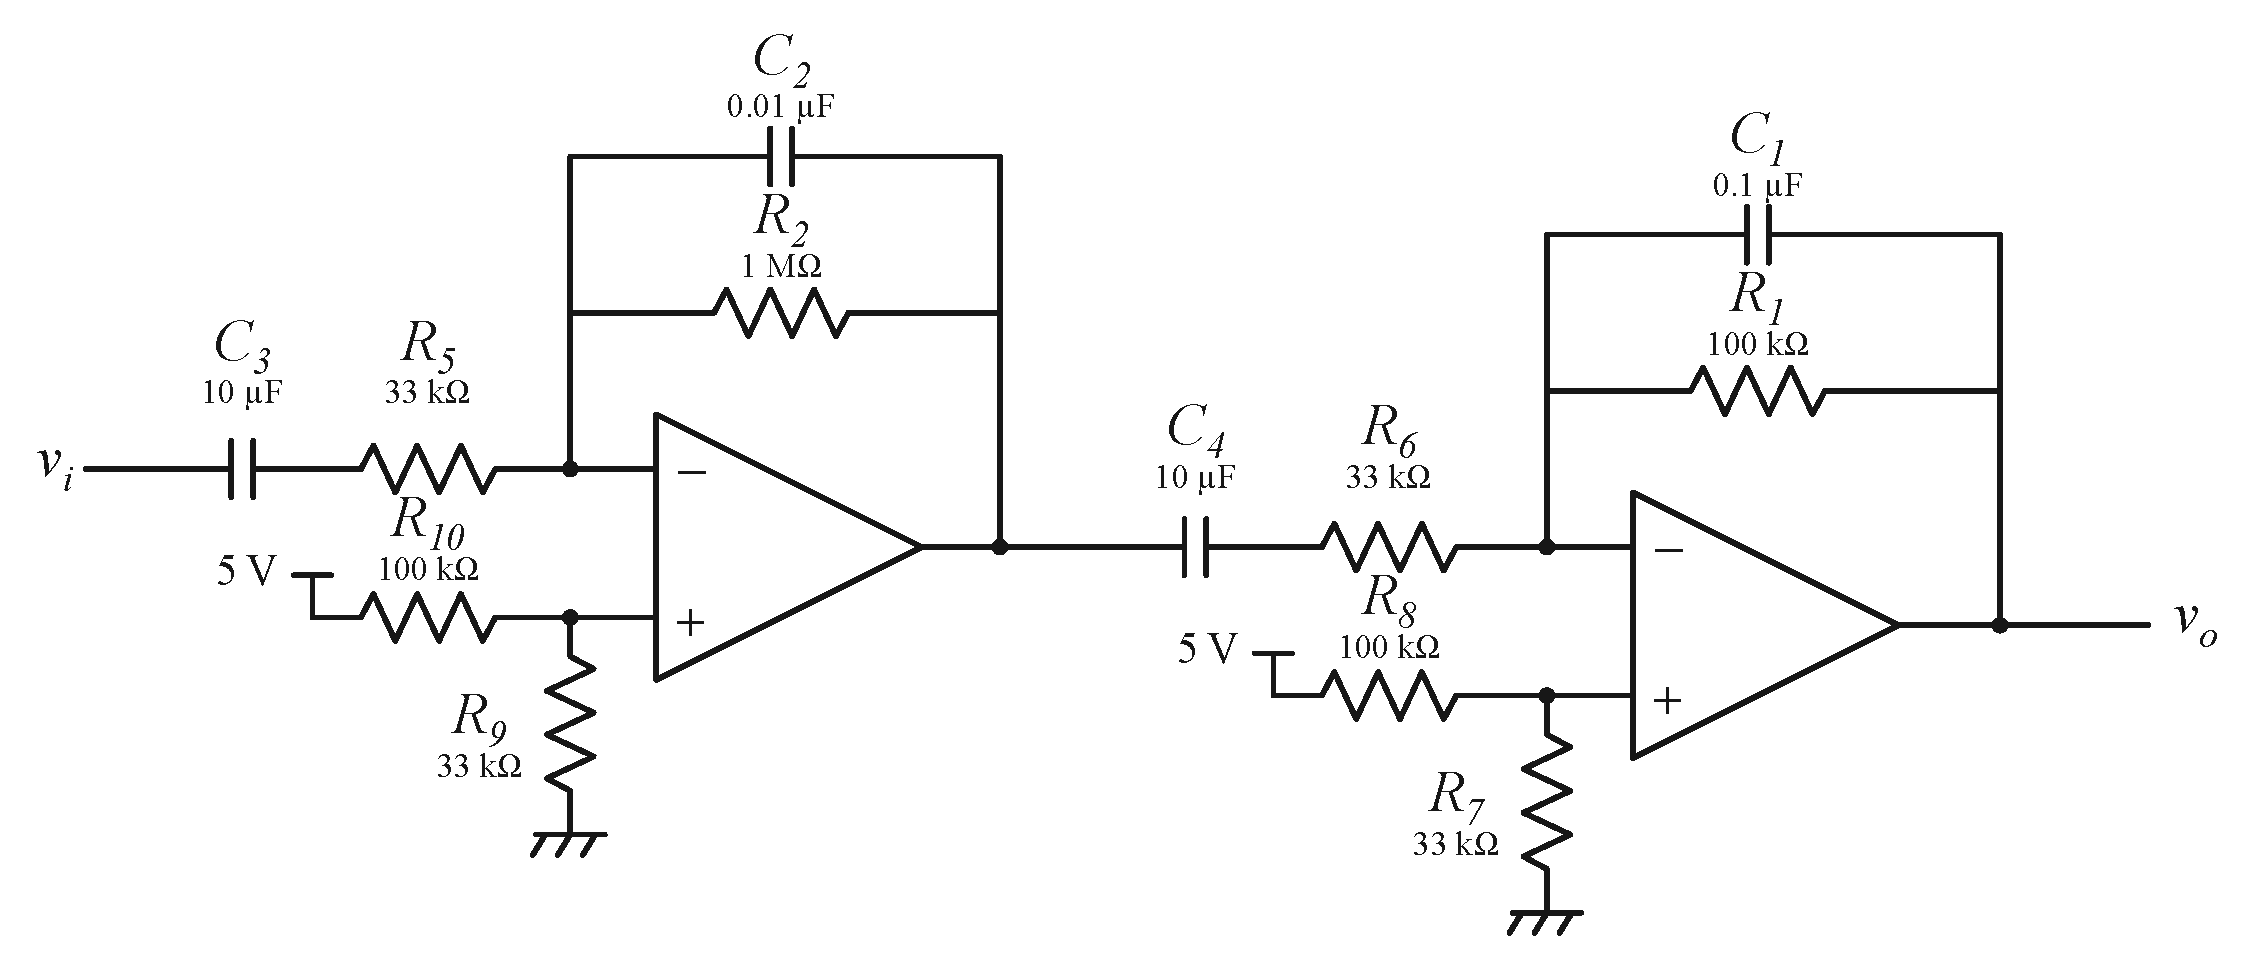
\includegraphics[width=0.9\textwidth,clip]{fig_work_A/circuit_diagram_A1.pdf}
  \caption{ワークA-1：ATOM Lite接続時のバンドパスフィルタ付き二段反転増幅回路図}
  \label{fig:circuit_schematic_A1}
\end{figure}

\begin{figure}[htbp]
  \centering
  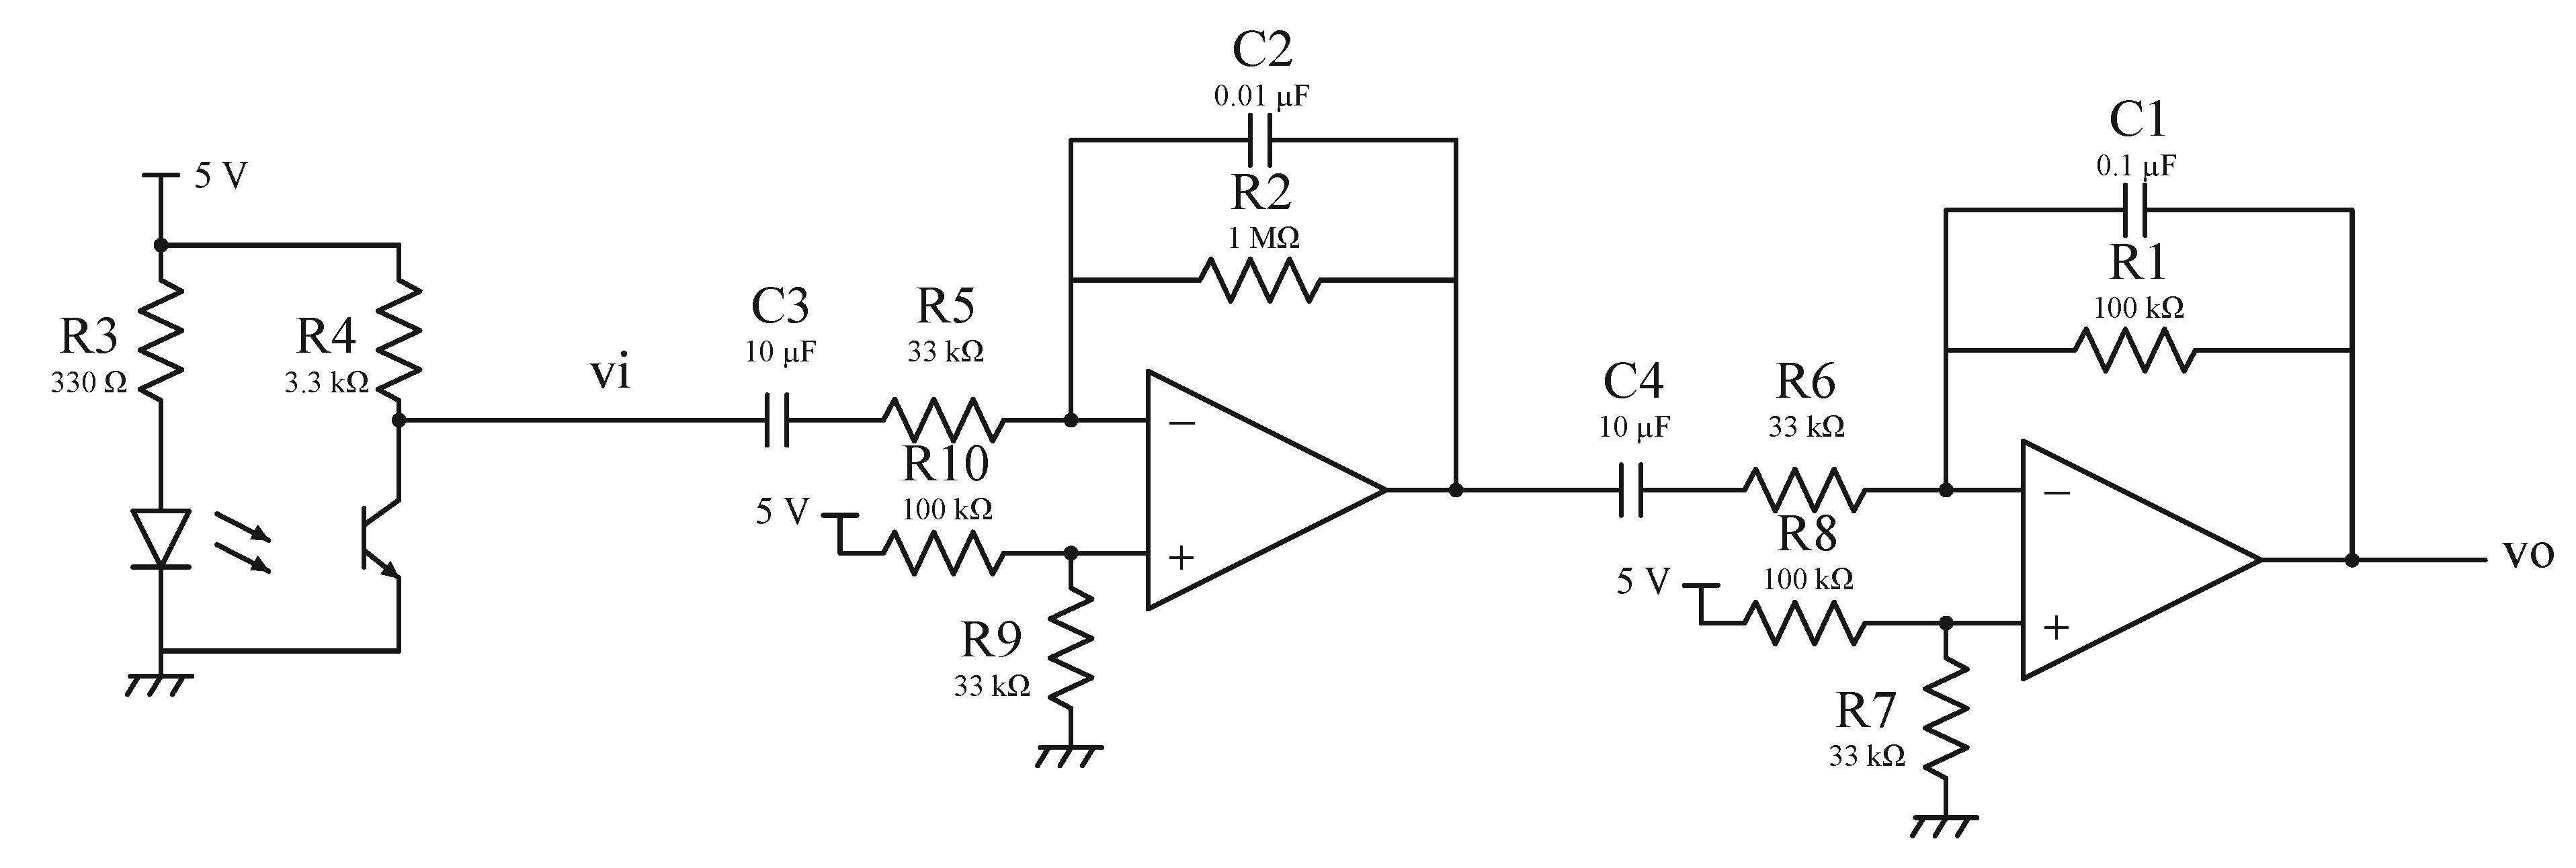
\includegraphics[width=0.9\textwidth,clip]{fig_work_A/circuit_diagram_A2.pdf}
  \caption{ワークA-2：脈拍検出部（フォトリフレクタ）を結合した全体回路図}
  \label{fig:circuit_schematic_A2}
\end{figure}

本回路は，図\ref{fig:circuit_schematic_A1}および図\ref{fig:circuit_schematic_A2}に示すように，主に「脈拍検出部（センサ部）」「初段反転増幅・フィルタ部」「後段反転増幅・フィルタ部」「バイアス電位生成部」の4つの機能ブロックで構成されている．表\ref{tab:circuit_components}に示した素子を用いた各ブロックの具体的な配置および接続関係は以下の通りである：
\begin{enumerate}
  \item \textbf{脈拍検出部（フォトリフレクタ回路）}：
        反射型フォトリフレクタ（LBR-127HLD）の赤外LED側アノード端子に電源5\,Vラインから電流制限抵抗 $R_3$（$330\,\Omega$）を直列に接続し，カソード端子をGNDに接地する．受光側のフォトトランジスタは，コレクタ端子に電源5\,Vラインから負荷抵抗 $R_4$（$3.3\,\mathrm{k}\Omega$）を接続し，エミッタ端子をGNDに接地する．このフォトトランジスタのコレクタ電位を入力端子 $v_i$ として後段の増幅回路へ入力する（図\ref{fig:circuit_schematic_A2}）．なお，ワークA-1では脈拍検出部の代わりに，ATOM Lite（ピンG25）からの模擬信号を $1\,\mathrm{M}\Omega$ の保護抵抗を直列に介して入力端子 $v_i$ に接続する（図\ref{fig:circuit_schematic_A1}）．

  \item \textbf{初段反転増幅・フィルタ部}：
        2回路入りオペアンプ LM358N の第1ユニットを使用する．入力端子 $v_i$ から直流カット用の結合コンデンサ $C_3$（$10\,\mu\mathrm{F}$）および入力抵抗 $R_5$（$33\,\mathrm{k}\Omega$）を直列に経由して，オペアンプの反転入力端子（$-$端子）に接続する．オペアンプの出力端子と反転入力端子の間には，帰還抵抗 $R_2$（$1\,\mathrm{M}\Omega$）と高周波減衰用の並列コンデンサ $C_2$（$0.01\,\mu\mathrm{F}$）による並列帰還回路を構成する．非反転入力端子（$+$端子）には，後述する分圧抵抗による基準バイアス電位を印加する．

  \item \textbf{後段反転増幅・フィルタ部}：
        LM358N の第2ユニットを使用する．初段オペアンプの出力端子から段間結合コンデンサ $C_4$（$10\,\mu\mathrm{F}$）および入力抵抗 $R_6$（$33\,\mathrm{k}\Omega$）を経由して，後段オペアンプの反転入力端子（$-$端子）に接続する．出力端子 $v_o$ と反転入力端子の間には，帰還抵抗 $R_1$（$100\,\mathrm{k}\Omega$）と並列コンデンサ $C_1$（$0.1\,\mu\mathrm{F}$）による並列帰還回路を設ける．非反転入力端子（$+$端子）には，初段と同様に分圧抵抗による基準バイアス電位を印加する．回路全体の最終出力電圧 $v_o$ は後段オペアンプの出力端子から取り出す．

  \item \textbf{電源供給およびバイアス電位生成部}：
        オペアンプ LM358N の電源ピンには単電源5\,VおよびGNDを供給する（$V_{CC} = 5\,\mathrm{V}, V_{EE} = \mathrm{GND}$）．単一電源駆動において交流信号の正負両振幅を波形クリップさせずに安定動作させるため，初段の非反転入力端子には $R_{10} = 100\,\mathrm{k}\Omega$ と $R_9 = 33\,\mathrm{k}\Omega$ による分圧回路，後段の非反転入力端子には $R_8 = 100\,\mathrm{k}\Omega$ と $R_7 = 33\,\mathrm{k}\Omega$ による分圧回路を接続し，それぞれ約1.24\,Vの中間バイアス基準電位を供給する．
\end{enumerate}


\subsection{回路の設計理論と定数決定}

上述の使用素子一覧および回路図に基づき，各部の動作原理，設計目標仕様，および回路定数の算出根拠を詳述する．

\subsubsection{脈拍検出部（フォトリフレクタ回路）の設計原理}

脈拍検出部には，赤外発光ダイオード（LED）とフォトトランジスタが一体化された反射型フォトリフレクタ（LBR-127HLD\cite{LBR-127HLD}）を用いた．
指先をセンサ受発光面に近接させると，赤外LEDから出射された光が皮下の動脈血等で散乱・反射され，その反射光がフォトトランジスタに入射する．
心臓の拍動により血管内の動脈血量が増加するとヘモグロビンによる光吸収が増加して反射光量が減少し，フォトトランジスタのコレクタ電流が減少してコレクタ電位（出力電位）は上昇する．
逆に，血流量が減少すると反射光量が増加してコレクタ電位は低下する．

フォトリフレクタの動作条件および回路定数は以下のように決定した：
\begin{enumerate}
  \item \textbf{赤外LEDの電流制限抵抗 $R_3$ の設定}：
        赤外LEDの順方向電圧の典型値は $V_F = 1.2 \sim 1.5\,\mathrm{V}$，順方向定格電流は $I_F = 20\,\mathrm{mA}$ である．電源電圧 $V_{CC} = 5\,\mathrm{V}$ において電流 $I_F = 20\,\mathrm{mA}$ を流すための抵抗値は，
        \begin{equation}
          R = \frac{V_{CC} - V_F}{I_F} \approx \frac{5.0 - 1.35}{0.02} \approx 182.5\,\Omega
          \label{eq:R3_calc}
        \end{equation}
        と算出される．本実習では，素子の発熱抑制および安全マージンを考慮し，計算値の約2倍弱にあたる標準抵抗値 $R_3 = 330\,\Omega$ を採用した．このときLEDに流れる順方向電流は約 $11\,\mathrm{mA}$ となる．

  \item \textbf{フォトトランジスタの負荷抵抗 $R_4$ の設定}：
        フォトトランジスタのコレクタ--エミッタ間飽和電圧は $V_{CE(\mathrm{sat})} \approx 0.4\,\mathrm{V}$ である．光照射時にコレクタ電流 $I_C \approx 2\,\mathrm{mA}$ が流れるとし，負荷抵抗 $R_4$ において $V_{CC} - V_{CE(\mathrm{sat})} \approx 4.6\,\mathrm{V}$ の電圧降下が生じるものと仮定すると，
        \begin{equation}
          R = \frac{4.6\,\mathrm{V}}{0.002\,\mathrm{A}} = 2.3\,\mathrm{k}\Omega
          \label{eq:R4_calc}
        \end{equation}
        となる．本実習では，感度向上および確実な電圧変化幅を得るため，計算値の約1.5倍弱にあたる標準抵抗値 $R_4 = 3.3\,\mathrm{k}\Omega$ を採用した．
\end{enumerate}

\subsubsection{バンドパスフィルタ付き二段反転増幅回路の設計}

センサ後段回路には，汎用オペアンプ（LM358N）を用いたバンドパスフィルタ付き二段反転増幅回路を設計・構成した．
生体脈波の周波数帯域は，安静時心拍数（60$\sim$100\,bpm）を中心に約0.5\,Hzから数Hz程度である．
このため，体動等の低周波ノイズを除去する下限遮断周波数 $f_L \approx 0.48\,\mathrm{Hz}$，および商用電源ノイズ（50/60\,Hz）を除去する上限遮断周波数 $f_U \approx 16\,\mathrm{Hz}$ を目標仕様として設定した．
また，入力信号振幅（約20\,mV）を後段のA/D変換に適した約1.8\,V程度まで増幅するため，総合増幅率を約90倍に設定した．

\paragraph{オペアンプの基礎理論と反転増幅回路の動作原理}
オペアンプ（Operational Amplifier: 演算増幅器）は，2つの入力端子（反転入力端子 $v_1$ および非反転入力端子 $v_2$）と1つの出力端子 $v_o$ を持つ差動増幅器であり，入出力関係は差動開ループ利得 $A$ を用いて $v_o = -A(v_1 - v_2)$ で表される．
回路理論における理想オペアンプは，以下の4つの条件を満たすものとして定義される：
\begin{enumerate}
  \item 差動利得が無限大（$A \to \infty$）
  \item 入力インピーダンスが無限大（$Z_i \to \infty$，二入力端子間に電流は流入しない）
  \item 出力インピーダンスがゼロ（$Z_o \to 0$，外部負荷に関わらず出力電圧を維持）
  \item 増幅可能な周波数帯域が無限大（直流から高周波まで平坦な利得特性）
\end{enumerate}
これに対し，本実験で使用した LM358N は汎用の2回路入りオペアンプであり，単一電源（$V_{CC} = 5\,\mathrm{V}, V_{EE} = \mathrm{GND}$）での動作が可能である一方，有限な開ループ利得や利得帯域幅積（GBW $\approx 1\,\mathrm{MHz}$），スルーレート等の制約を有するアクティブ素子である．

オペアンプの出力端子から反転入力端子へ帰還抵抗 $R_f$ を介して出力信号の一部を戻す構成を「負帰還（Negative Feedback）」と呼ぶ．
負帰還が施された回路において，入力電圧 $v_i$ が上昇すると出力 $v_o$ は下降し，この出力下降分が直ちに $R_f$ を通じて反転入力端子へと帰還されるため，$v_i$ の上昇が抑制される．
この自己補正作用と開ループ利得 $A \to \infty$ の特性により，二入力端子間の電位差は極めて微小となり，平衡状態において二入力端子の電位は等しくなる（$v_1 = v_2$）．
これを「仮想短絡（バーチャルショート: Virtual Short）」と呼ぶ．
仮想短絡においては，両端子間があたかも短絡（ショート）しているように電位が等しく維持されるが，入力インピーダンス $Z_i \to \infty$ であるため入力端子内部へ電流が流れ込むことはない（$i = 0$）．

反転増幅器の利得導出は以下の通りである．非反転入力端子に基準電位（接地の場合は 0\,V）が与えられているとき，仮想短絡により反転入力端子の電位も基準電位と等しくなる．
入力抵抗 $R_s$ を流れる電流を $i$ とすると，入力端子間の電流流入がゼロであるため，キルヒホッフの電流則より $i$ の全量が帰還抵抗 $R_f$ へと流れる．
したがって，入力側にかかる電圧降下 $v_1$ および帰還抵抗の両端電圧 $v_2$ はオームの法則より，
\begin{equation}
  i = \frac{v_1}{R_s} = \frac{v_2}{R_f}
  \label{eq:inverting_kcl}
\end{equation}
となる．仮想短絡により入力電位は $v_i = v_1$ であり，出力電位は反転入力端子より $v_2$ だけ低下するため，
\begin{equation}
  v_o = -v_2 = -R_f i = -\frac{R_f}{R_s} v_1 = -\frac{R_f}{R_s} v_i
  \label{eq:inverting_gain_proof}
\end{equation}
となり，閉ループ増幅率 $A_f = -R_f / R_s$ が厳密に導出される．

\paragraph{バンドパスフィルタ機能の付加}
本実習では，この反転増幅回路に入力結合コンデンサ $C_s$ および帰還並列コンデンサ $C_f$ を付加し，周波数選択性を持たせた．
入力側の結合容量 $C_s$ は直流成分（0\,Hz）を完全に遮断し，低周波ノイズを除去する1次ハイパスフィルタ（HPF）を形成する．その下限遮断周波数 $f_L$ は，
\begin{equation}
  f_L = \frac{1}{2\pi C_s R_s}
  \label{eq:fl_theory}
\end{equation}
で決定される．一方，帰還抵抗 $R_f$ に並列接続されたコンデンサ $C_f$ は，高周波においてインピーダンス $1/(2\pi f C_f)$ が低下して実効的な帰還インピーダンスを低下させるため，高周波利得を減衰させる1次ローパスフィルタ（LPF）として機能する．その上限遮断周波数 $f_U$ は，
\begin{equation}
  f_U = \frac{1}{2\pi C_f R_f}
  \label{eq:fu_theory}
\end{equation}
となる．これにより，通過帯域（$f_L \ll f \ll f_U$）において所定の反転増幅率 $-R_f / R_s$ を示しつつ，不要な超低周波および高周波を減衰させるバンドパス特性が得られる．

\paragraph{各増幅段の具体的な回路定数および設計値}
回路図（図\ref{fig:circuit_schematic_A1}, \ref{fig:circuit_schematic_A2}）に示した各素子の具体的な回路定数および設計値は以下の通りである：

\begin{enumerate}
  \item \textbf{初段反転増幅回路（$-30.30$倍）}：
        入力側に結合コンデンサ $C_3$ と入力抵抗 $R_5$，オペアンプの帰還路に抵抗 $R_2$ と並列コンデンサ $C_2$ を接続した．
        \begin{itemize}
          \item \textbf{中域理論増幅率 $A_{v1}$}：帰還抵抗 $R_2 = 1\,\mathrm{M}\Omega$，入力抵抗 $R_5 = 33\,\mathrm{k}\Omega$ により，
                \begin{equation}
                  A_{v1} = -\frac{R_2}{R_5} = -\frac{1.0 \times 10^6}{33 \times 10^3} \approx -30.30\,\text{倍}
                  \label{eq:gain1}
                \end{equation}
          \item \textbf{下限遮断周波数 $f_{L1}$（HPF特性）}：$C_3 = 10\,\mu\mathrm{F}$，$R_5 = 33\,\mathrm{k}\Omega$ により，
                \begin{equation}
                  f_{L1} = \frac{1}{2\pi C_3 R_5} = \frac{1}{2\pi \times (10 \times 10^{-6}) \times (33 \times 10^3)} \approx 0.482\,\mathrm{Hz}
                  \label{eq:fl1}
                \end{equation}
          \item \textbf{上限遮断周波数 $f_{U1}$（LPF特性）}：$C_2 = 0.01\,\mu\mathrm{F}$，$R_2 = 1\,\mathrm{M}\Omega$ により，
                \begin{equation}
                  f_{U1} = \frac{1}{2\pi C_2 R_2} = \frac{1}{2\pi \times (0.01 \times 10^{-6}) \times (1.0 \times 10^6)} \approx 15.92\,\mathrm{Hz}
                  \label{eq:fu1}
                \end{equation}
          \item \textbf{バイアス回路}：非反転入力端子には $R_{10} = 100\,\mathrm{k}\Omega$ と $R_9 = 33\,\mathrm{k}\Omega$ による分圧回路を接続し，基準電位 $V_{\mathrm{ref1}} = 5\,\mathrm{V} \times \frac{33}{100 + 33} \approx 1.24\,\mathrm{V}$ を与えた．
        \end{itemize}

  \item \textbf{後段反転増幅回路（$-3.030$倍）}：
        初段出力からの結合コンデンサ $C_4$ と入力抵抗 $R_6$，帰還抵抗 $R_1$ と並列コンデンサ $C_1$ を接続した．
        \begin{itemize}
          \item \textbf{中域理論増幅率 $A_{v2}$}：帰還抵抗 $R_1 = 100\,\mathrm{k}\Omega$，入力抵抗 $R_6 = 33\,\mathrm{k}\Omega$ により，
                \begin{equation}
                  A_{v2} = -\frac{R_1}{R_6} = -\frac{100 \times 10^3}{33 \times 10^3} \approx -3.030\,\text{倍}
                  \label{eq:gain2}
                \end{equation}
          \item \textbf{下限遮断周波数 $f_{L2}$（HPF特性）}：$C_4 = 10\,\mu\mathrm{F}$，$R_6 = 33\,\mathrm{k}\Omega$ により，
                \begin{equation}
                  f_{L2} = \frac{1}{2\pi C_4 R_6} \approx 0.482\,\mathrm{Hz}
                  \label{eq:fl2}
                \end{equation}
          \item \textbf{上限遮断周波数 $f_{U2}$（LPF特性）}：$C_1 = 0.1\,\mu\mathrm{F}$，$R_1 = 100\,\mathrm{k}\Omega$ により，
                \begin{equation}
                  f_{U2} = \frac{1}{2\pi C_1 R_1} = \frac{1}{2\pi \times (0.1 \times 10^{-6}) \times (100 \times 10^3)} \approx 15.92\,\mathrm{Hz}
                  \label{eq:fu2}
                \end{equation}
          \item \textbf{バイアス回路}：非反転入力端子には $R_8 = 100\,\mathrm{k}\Omega$ と $R_7 = 33\,\mathrm{k}\Omega$ による分圧回路を接続し，基準電位 $V_{\mathrm{ref2}} \approx 1.24\,\mathrm{V}$ を与えた．
        \end{itemize}

  \item \textbf{回路全体の総合特性と理論モデル}：
        二段の反転増幅器を直列接続することにより，通過帯域中域における公称総合利得 $A_v$ は，
        \begin{equation}
          A_v = A_{v1} \times A_{v2} = (-30.30) \times (-3.030) \approx +91.8\,\text{倍}
          \label{eq:total_gain}
        \end{equation}
        となる．
        反転増幅を2回繰り返すため，中域における静的な信号極性は非反転（正の利得）となる．
        ただし，回路各段にHPFおよびLPFが含まれるため，周波数 $f$ における回路全体の理想振幅伝達関数 $|H(f)|$ は次式で与えられる：
        \begin{equation}
          |H(f)| = A_v \cdot \frac{1}{1 + (f_L/f)^2} \cdot \frac{1}{1 + (f/f_U)^2}
          \label{eq:amplitude_transfer}
        \end{equation}
        ここで $f_L \approx 0.482\,\mathrm{Hz}$，$f_U \approx 15.92\,\mathrm{Hz}$ である．この振幅伝達関数より，通過帯域内であっても遮断周波数近傍では利得が低下する．
        また，回路全体の理論位相特性 $\phi(f)$ および理論群遅延 $\tau_g(f)$ はそれぞれ，
        \begin{equation}
          \phi(f) \approx 2 \left( \arctan\frac{f_L}{f} - \arctan\frac{f}{f_U} \right) \quad [\mathrm{rad}]
          \label{eq:phase_transfer}
        \end{equation}
        \begin{equation}
          \tau_g(f) = -\frac{1}{2\pi}\frac{d\phi(f)}{df} = \frac{1}{\pi} \left( \frac{f_L}{f^2 + f_L^2} + \frac{f_U}{f^2 + f_U^2} \right) \quad [\mathrm{s}]
          \label{eq:group_delay_transfer}
        \end{equation}
        で表される．ここで，初段および後段の帰還RC時定数はそれぞれ $R_2 C_2 = 1\,\mathrm{M}\Omega \times 0.01\,\mu\mathrm{F} = 10.0\,\mathrm{ms}$，$R_1 C_1 = 100\,\mathrm{k}\Omega \times 0.1\,\mu\mathrm{F} = 10.0\,\mathrm{ms}$ であり，その和である約20.0\,msは高周波（LPF部）のみに着目した低周波極限近似値に相当し，全回路群遅延式(\ref{eq:group_delay_transfer})とは異なる点に留意が必要である．

        さらに，炭素皮膜抵抗器（金色帯，許容差 $\pm 5\%$）の公差を考慮した最悪条件（帰還抵抗 $-5\%$，入力抵抗 $+5\%$）における利得下限値は，
        \begin{align}
          A_{v1,\min} &= -\frac{R_2 \times (1 - 0.05)}{R_5 \times (1 + 0.05)} = -\frac{950\,\mathrm{k}\Omega}{34.65\,\mathrm{k}\Omega} \approx -27.42\,\text{倍} \label{eq:gain1_min} \\
          A_{v2,\min} &= -\frac{R_1 \times (1 - 0.05)}{R_6 \times (1 + 0.05)} = -\frac{95.0\,\mathrm{k}\Omega}{34.65\,\mathrm{k}\Omega} \approx -2.742\,\text{倍} \label{eq:gain2_min} \\
          A_{v,\min}  &= A_{v1,\min} \times A_{v2,\min} = (-27.42) \times (-2.742) \approx +75.19\,\text{倍} \label{eq:total_gain_min}
        \end{align}
        と算定される．なお，ATOM Lite の DAC 出力と回路入力端子の間に挿入された保護用直列抵抗 $R_{\mathrm{ext}} = 1\,\mathrm{M}\Omega$ は回路入力インピーダンス（初段 $R_5$）との間で分圧減衰比 $\alpha \approx R_5 / (R_{\mathrm{ext}} + R_5) \approx 0.032$ を生じさせるが，オシロスコープのCH1プローブは $R_{\mathrm{ext}}$ の後段にあたる入力端子 $v_i$ に接続されているため，$v_i$ そのものが回路への実入力振幅として観測され，測定される増幅率 $v_o / v_i$ にはこの分圧比は影響しない．
\end{enumerate}


\subsection{実験手順}

実験は以下の二段階の手順に沿って実施した．

\subsubsection{ワークA-1：二段反転増幅回路の作成と周波数特性評価}
\begin{enumerate}
  \item ブレッドボード上にオペアンプ LM358N，抵抗器，コンデンサを配置し，図\ref{fig:circuit_schematic_A1}に示すバンドパスフィルタ付き二段反転増幅回路を配線した．電源ラインには安定化電源より5\,VおよびGNDを供給した．
  \item 模擬信号発生器として ATOM Lite を用意し，信号出力ピン（G25）と増幅回路の入力端子 $v_i$ の間に $1\,\mathrm{M}\Omega$ の抵抗を直列に挿入して接続した．
  \item ATOM Lite から以下の4種類の信号を順次入力した：
        \begin{itemize}
          \item \textbf{波形1（緑）}：低周波正弦波（公称1\,Hz）
          \item \textbf{波形2（赤）}：低周波正弦波（公称1\,Hz）と高周波正弦波（公称100\,Hz）の合成波
          \item \textbf{波形3（青）}：低周波正弦波（公称1\,Hz）と高周波正弦波（公称7\,Hz）の合成波
          \item \textbf{波形4（紫）}：模擬脈波
        \end{itemize}
  \item デジタルオシロスコープのプローブ CH1 を入力端子 $v_i$ に，CH2 を出力端子 $v_o$ にそれぞれ接続した．
  \item オシロスコープの設定を以下のように調整した：
        \begin{itemize}
          \item 水平系：\texttt{Acquire} $\rightarrow$ \texttt{Mode} を「\texttt{Hi-res}（高分解能）」に設定．
          \item 垂直系：CH1 および CH2 のカップリング設定を「\texttt{AC}（交流結合）」に設定．
        \end{itemize}
  \item 各波形について，オシロスコープの測定レンジおよび目盛り読み取り値を記録し，画面波形を画像ファイルとして保存した．
\end{enumerate}

\subsubsection{ワークA-2：脈拍検出回路の作成と脈波計測}
\begin{enumerate}
  \item ブレッドボード上にフォトリフレクタ LBR-127HLD を配置し，赤外LED側に電流制限抵抗 $R_3$（$330\,\Omega$），フォトトランジスタ側に負荷抵抗 $R_4$（$3.3\,\mathrm{k}\Omega$）を接続して脈拍検出回路を構成した（図\ref{fig:circuit_schematic_A2}）．
  \item フォトトランジスタのコレクタ端子を，作成した二段反転増幅回路の入力端子 $v_i$ に接続した．
  \item フォトリフレクタの受発光面に被験者の人差し指の腹を軽く当て，過度な圧迫とならないよう静置した．
  \item オシロスコープにて出力端子 $v_o$（CH2）の波形を観測し，脈動に伴う明瞭な脈波ピークが得られるよう指の配置・接触圧を微調整した．
  \item 安定した脈波波形を観測した状態でオシロスコープの画面を静止（Stop）させ，波形画像を保存した．
  \item 保存した波形から，最も周期が長い波形区間，および次に長い波形区間を選定し，時間軸目盛り，電圧軸目盛り，測定レンジ等の諸元を記録した．
\end{enumerate}

\begin{figure}[htbp]
  \centering
  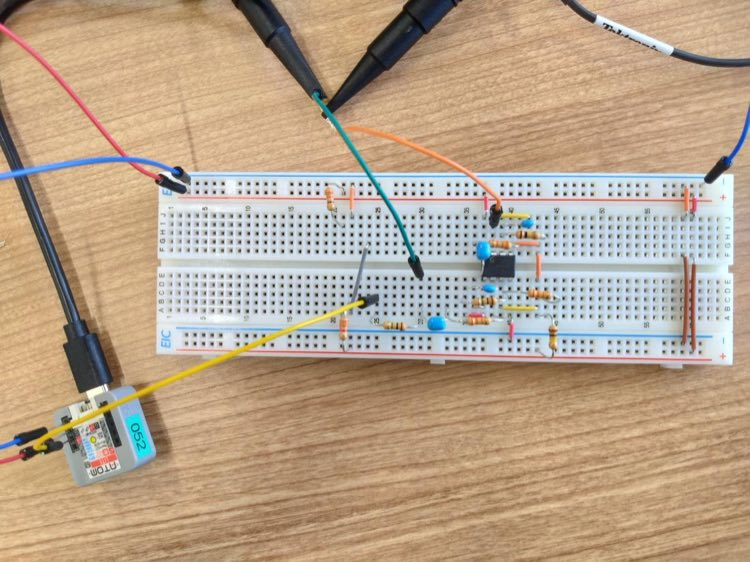
\includegraphics[width=0.75\textwidth,clip]{fig_work_A/回路.jpg}
  \caption{ブレッドボード上に実装したバンドパスフィルタ付き二段反転増幅回路の実物外観}
  \label{fig:implemented_circuit}
\end{figure}


%-----------------------------------------------------------------------------------
\section{結果}
%% 実験から得られた結果を，目的や方法を理解した上で，重要データを外す
%% ことなく，要領よくまとめてください．
%%
%% 結果（数値）は，（自分はポイントを理解しているということをアピール
%% しながら）視認性（一覧性）を高めて報告することが求められる．この意
%% 味で，要領よくまとめられた表が望ましい．決して，文章の中にバラバラ
%% に埋没させて，読み手がどこに書いているか分かりにくい（書き手にとっ
%% ては都合のよい）記載するものではない点に注意する．

\subsection{ワークA-1：波形出力デバイス入力時の測定結果}

ATOM Lite から4種類のテスト波形を入力した際のオシロスコープ設定パラメータおよび目盛り読み取り諸元を表\ref{tab:result_raw_work_A1}に示す．
また，これらに基づき算出した周期，周波数，振幅，増幅率，時間差，および入出力位相差を表\ref{tab:result_calc_work_A1}に示す．
各入力波形におけるオシロスコープの全体観測画面（低周波観測，200\,ms/div）を図\ref{fig:waveforms_work_A1}に示す．
また，重畳された高周波成分の拡大観測，および信号立ち上がり時における過渡応答の拡大観測画面を図\ref{fig:waveforms_work_A1_zoom}に示す．
各波形画面上には，波形のピーク・谷底および信号変化点を明確に示すカーソル線（白色破線），測定区間を示す寸法線，ならびに読み取った目盛り幅（div値）を付記し，計測根拠の客観性と視認性を高めた．
立ち上がり過渡応答の拡大観測（図\ref{fig:waveforms_work_A1_zoom}(c), (d)）に着目すると，いずれの波形においても入力信号 $v_i$（CH1：黄）が先行して変化し，出力信号 $v_o$（CH2：水色）が遅れて応答している様子が確認できる．
入出力信号間の時間差 $\Delta t$ および低周波周期 $T$ に基づく形式的な位相換算値 $\theta$ は，出力の入力に対する遅延を負値として，
\begin{equation}
  \theta = -\frac{\Delta t}{T} \times 2\pi \quad [\mathrm{rad}]
  \label{eq:phase_calc_result}
\end{equation}
により算出した．
表\ref{tab:result_raw_work_A1}には，低周波観測，高周波拡大観測，過渡時間差観測の各測定フェーズに対応する計器レンジ設定と目盛り読み取り値を整理して記録した．また，表\ref{tab:result_calc_work_A1}には，これらに基づく実時間・実電圧・実測周波数・増幅率・位相換算値を記録した．電圧振幅はすべてピーク間電圧（$V_{\mathrm{pp}}$）として定義している．

\begin{table}[htbp]
  \caption{波形出力デバイス入力時におけるオシロスコープ測定値および設定一覧}
  \centering
  \resizebox{\textwidth}{!}{%
    \begin{tabular}{|c||c|c|c|c|c|c||c|c|c|c|c|c||c|c|}
      \hline
      \multirow{3}{*}{入力波形}  & \multicolumn{6}{c||}{低周波観測（全体観測）} & \multicolumn{6}{c||}{高周波拡大観測} & \multicolumn{2}{c|}{過渡時間差観測} \\
      \cline{2-15}
                             & TIME/DIV & CH1 VOLT & CH2 VOLT & 周期 & CH1 $V_{i,\mathrm{pp}}$ & CH2 $V_{o,\mathrm{pp}}$ & TIME/DIV & CH1 VOLT & CH2 VOLT & 周期 & CH1 $V_{i,\mathrm{pp}}$ & CH2 $V_{o,\mathrm{pp}}$ & TIME/DIV & 時間差 $\Delta t$ \\
                             & [ms/div] & [mV/div] & [mV/div] & [div] & [div] & [div] & [ms/div] & [mV/div] & [mV/div] & [div] & [div] & [div] & [ms/div] & [div] \\
      \hline\hline
      波形1（1\,Hz正弦波）          & 200      & 10.0     & 100      & 3.3  & 2.0  & 9.4  & ---      & ---      & ---      & ---  & ---  & ---  & 0.400    & 0.15           \\
      \hline
      波形2（1\,Hz $+$ 100\,Hz） & 200      & 10.0     & 500      & 3.4  & 3.5  & 2.0  & 40.0     & 10.0     & 500      & 2.0  & 1.8  & 1.0  & 40.0     & 0.44           \\
      \hline
      波形3（1\,Hz $+$ 7\,Hz）   & 200      & 10.0     & 200      & 3.5  & 3.2  & 5.4  & 100      & 10.0     & 200      & 0.8  & 1.6  & 1.0  & 40.0     & 0.50           \\
      \hline
      波形4（模擬脈波）              & 200      & 10.0     & 500      & 4.4  & 4.2  & 4.3  & 40.0     & 10.0     & 500      & 6.5  & ---  & ---  & 200      & 0.15           \\
      \hline
    \end{tabular}%
  }
  \vspace{0.2em}
  {\footnotesize \raggedright ※低周波観測における電圧振幅は合成波全体のピーク間値（div）を表す．時間差 $\Delta t$ は立ち上がり時の入出力波形時間差拡大観測における読み取り値（波形4は低周波全体観測における読み取り値）を表す．\par}
  \label{tab:result_raw_work_A1}
\end{table}

\begin{table}[htbp]
  \caption{波形出力デバイス入力時における算定諸特性一覧}
  \centering
  \resizebox{\textwidth}{!}{%
    \begin{tabular}{|c||c|c|c|c|c||c|c|c|c||c|c|}
      \hline
      \multirow{3}{*}{入力波形}  & \multicolumn{5}{c||}{低周波信号（全体特性）} & \multicolumn{4}{c||}{高周波拡大観測成分} & \multicolumn{2}{c|}{過渡時間差・位相換算} \\
      \cline{2-12}
                             & 周期 $T$ & 実測周波数 $f$ & $V_{i,\mathrm{pp}}$ & $V_{o,\mathrm{pp}}$ & 振幅比 $A_v$ & 周期 $T_{\mathrm{high}}$ & 実測周波数 $f_{\mathrm{high}}$ & $V_{i,\mathrm{pp}}$ & $V_{o,\mathrm{pp}}$ & 時間差 $\Delta t$ & 位相換算 $\theta$ \\
                             & [ms]    & [Hz]          & [mV]                 & [mV]                 & $V_{o}/V_{i}$ [倍] & [ms] & [Hz] & [mV] & [mV] & [ms] & [rad] \\
      \hline\hline
      波形1（1\,Hz正弦波）          & 660     & 1.52          & 20.0                 & 940                  & 47.0         & ---  & ---  & ---  & ---  & 0.060             & $-0.0006$         \\
      \hline
      波形2（1\,Hz $+$ 100\,Hz） & 680     & 1.47          & 35.0                 & 1000                 & 28.6         & 80.0 & 12.5 & 18.0 & 500  & 17.6              & $-0.163$          \\
      \hline
      波形3（1\,Hz $+$ 7\,Hz）   & 700     & 1.43          & 32.0                 & 1080                 & 33.8         & 80.0 & 12.5 & 16.0 & 200  & 20.0              & $-0.180$          \\
      \hline
      波形4（模擬脈波）              & 880     & 1.14          & 42.0                 & 2150                 & 51.2         & 260.0& 3.85 & ---  & ---  & 30.0              & $-0.214$          \\
      \hline
    \end{tabular}%
  }
  \vspace{0.2em}
  {\footnotesize \raggedright ※波形2・3・4の低周波振幅比 $A_v$ は合成波全体のピーク間電圧比 $V_{o,\mathrm{pp}} / V_{i,\mathrm{pp}}$ を示す．位相換算値 $\theta$ は過渡時間差 $\Delta t$ と低周波周期 $T$ から式(\ref{eq:phase_calc_result})により算出した値である．\par}
  \label{tab:result_calc_work_A1}
\end{table}

\begin{figure}[htbp]
  \centering
  \begin{minipage}[b]{0.48\textwidth}
    \centering
    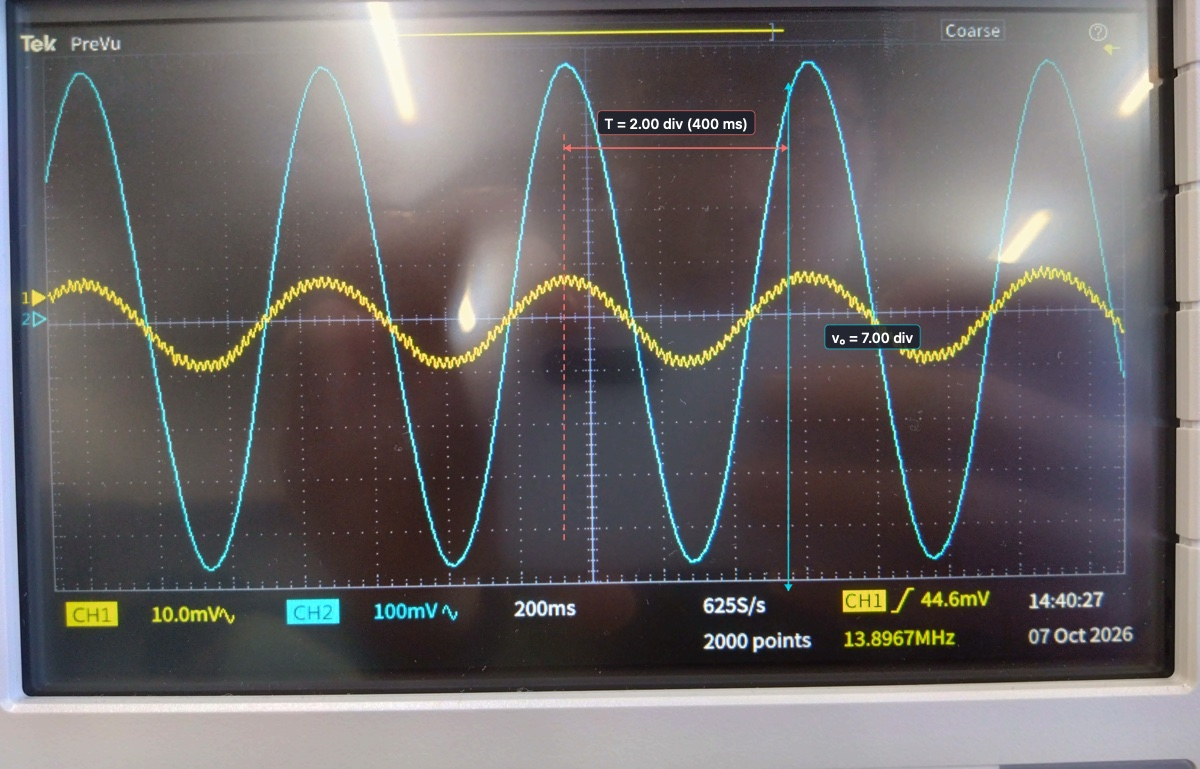
\includegraphics[width=\textwidth,clip]{fig_work_A/緑.jpg}
    \caption{波形1（1\,Hz正弦波）の入出力波形}
    \label{fig:wave1}
  \end{minipage}
  \hfill
  \begin{minipage}[b]{0.48\textwidth}
    \centering
    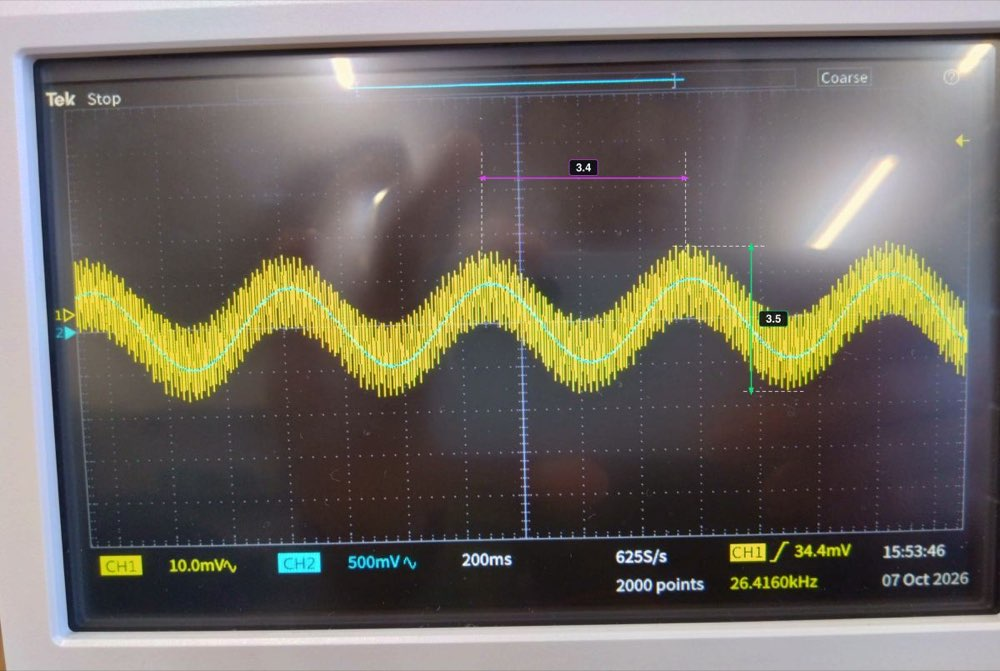
\includegraphics[width=\textwidth,clip]{fig_work_A/赤.jpg}
    \caption{波形2（1\,Hz $+$ 100\,Hz）の入出力波形}
    \label{fig:wave2}
  \end{minipage}
  \vspace{0.8em}
  \begin{minipage}[b]{0.48\textwidth}
    \centering
    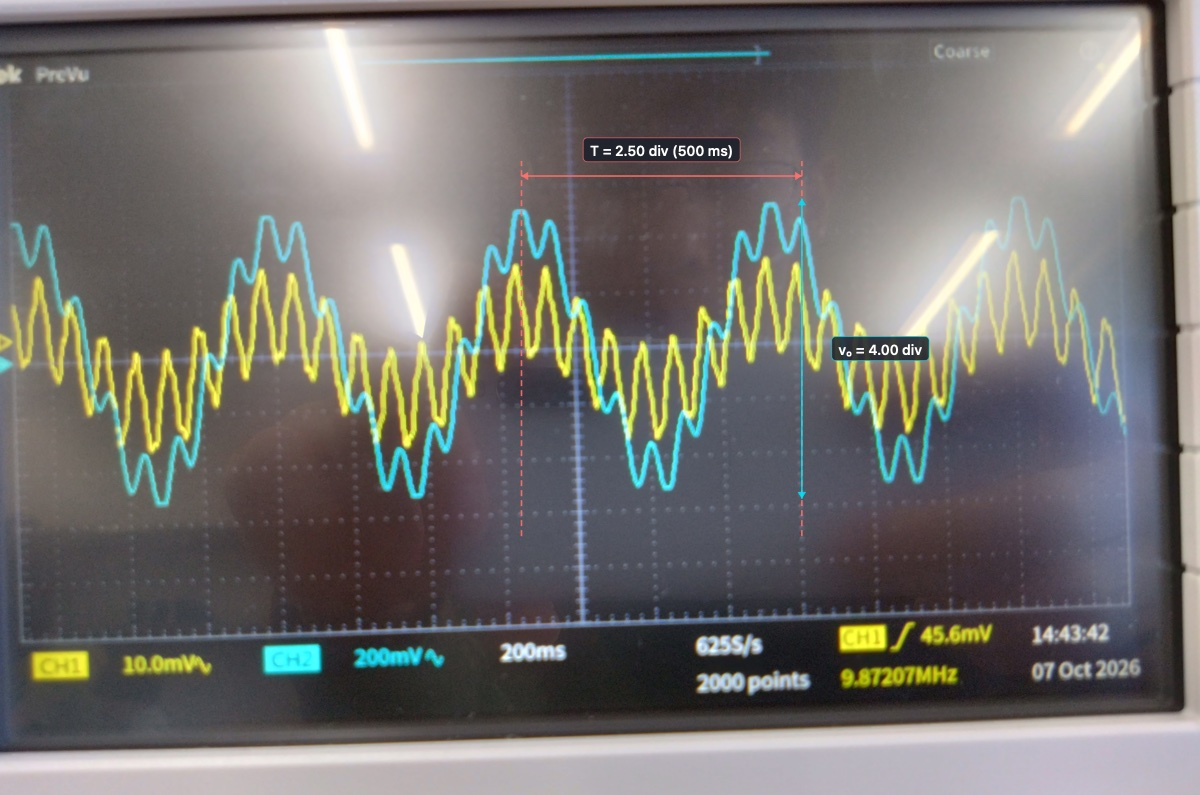
\includegraphics[width=\textwidth,clip]{fig_work_A/青.jpg}
    \caption{波形3（1\,Hz $+$ 7\,Hz）の入出力波形}
    \label{fig:wave3}
  \end{minipage}
  \hfill
  \begin{minipage}[b]{0.48\textwidth}
    \centering
    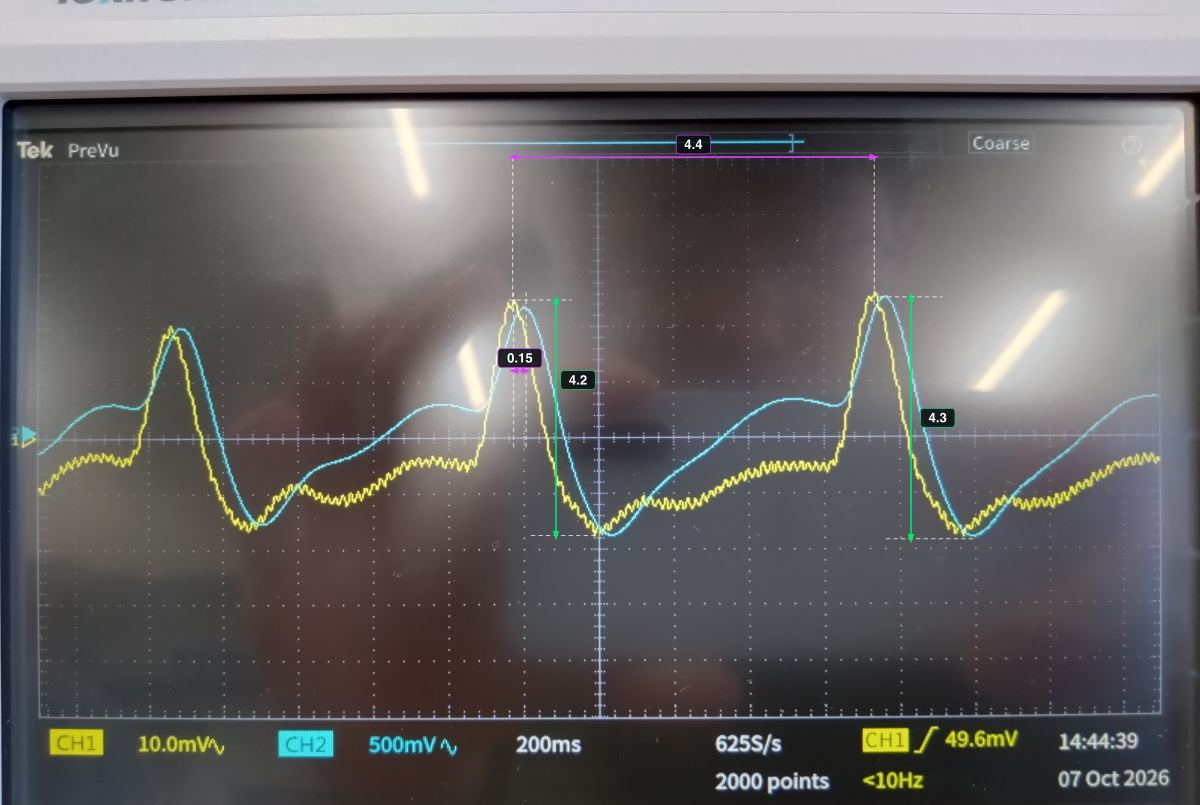
\includegraphics[width=\textwidth,clip]{fig_work_A/紫.jpg}
    \caption{波形4（模擬脈波）の入出力波形}
    \label{fig:wave4}
  \end{minipage}
  \caption{オシロスコープによる波形出力デバイスの低周波全体観測波形（CH1：$v_i$［黄］，CH2：$v_o$［水色］）}
  \label{fig:waveforms_work_A1}
\end{figure}

\begin{figure}[htbp]
  \centering
  \begin{minipage}[b]{0.48\textwidth}
    \centering
    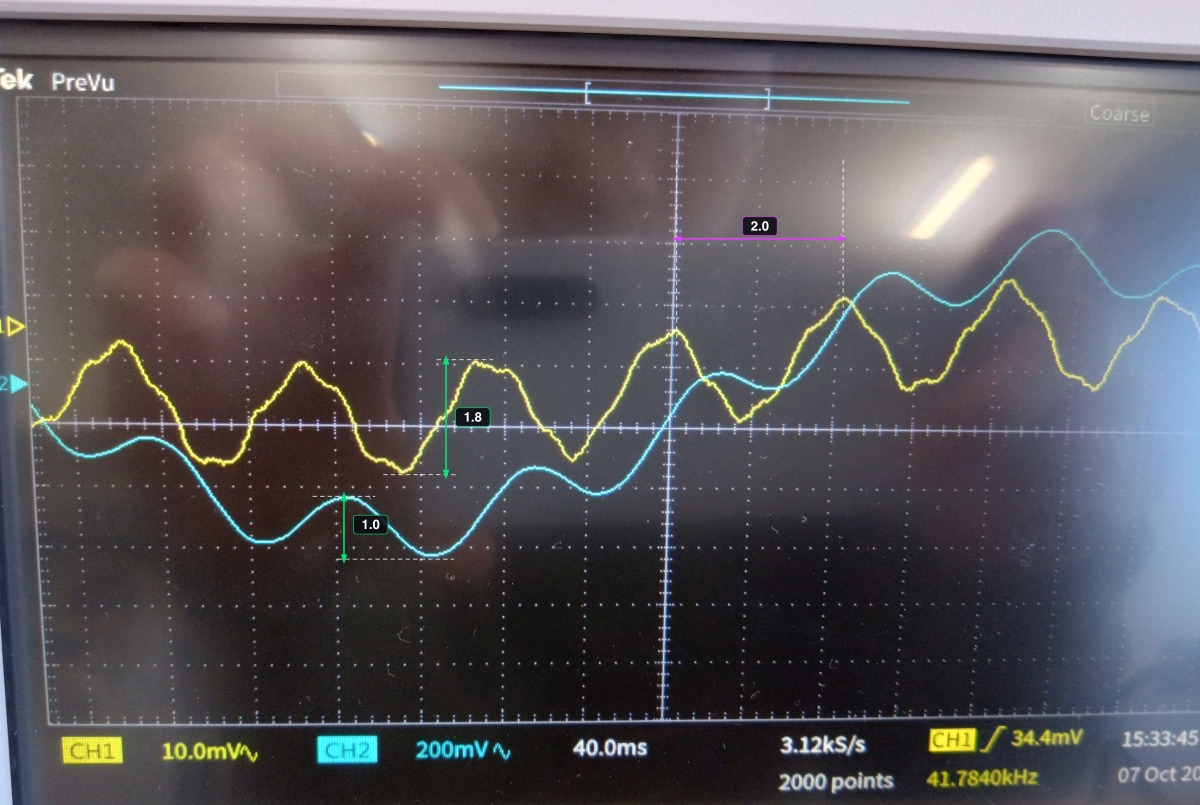
\includegraphics[width=\textwidth,clip]{fig_work_A/赤高.jpg}
    \caption{波形2 高周波成分（100\,Hz）の拡大観測}
    \label{fig:wave2_high}
  \end{minipage}
  \hfill
  \begin{minipage}[b]{0.48\textwidth}
    \centering
    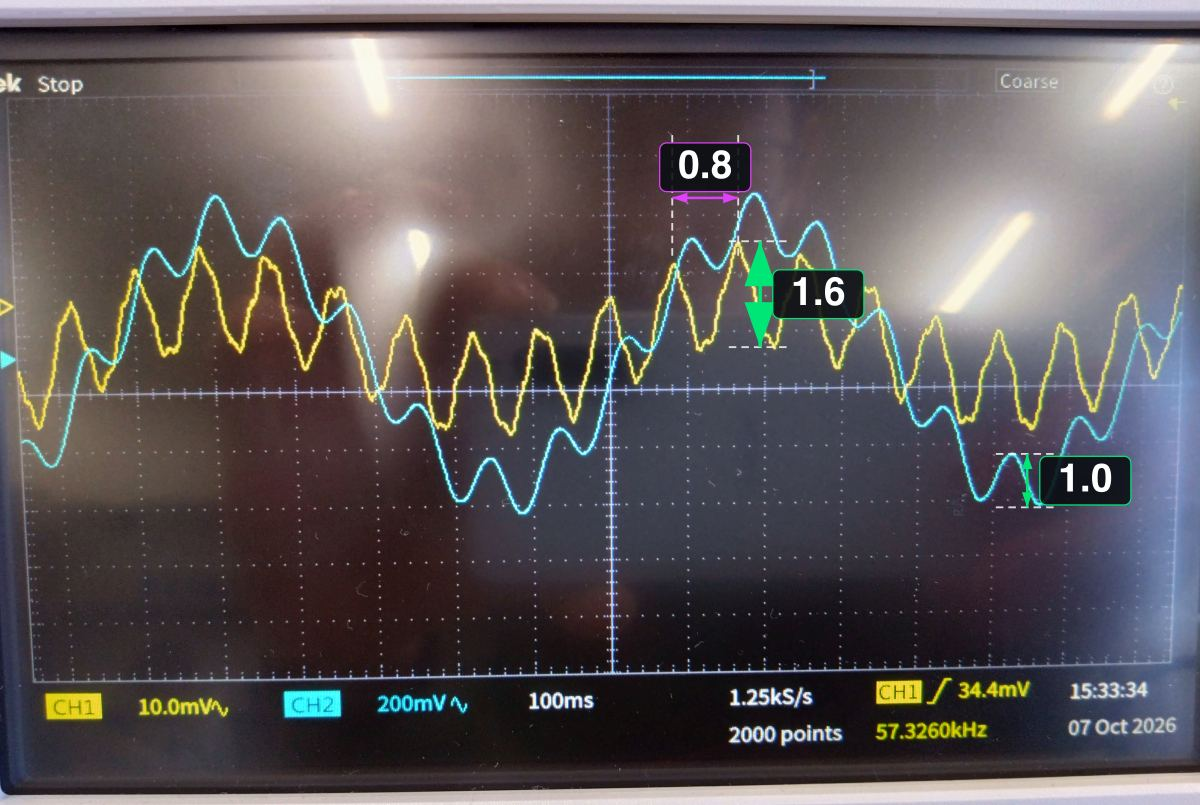
\includegraphics[width=\textwidth,clip]{fig_work_A/青高.jpg}
    \caption{波形3 高周波成分（7\,Hz）の拡大観測}
    \label{fig:wave3_high}
  \end{minipage}
  \vspace{0.8em}
  \begin{minipage}[b]{0.48\textwidth}
    \centering
    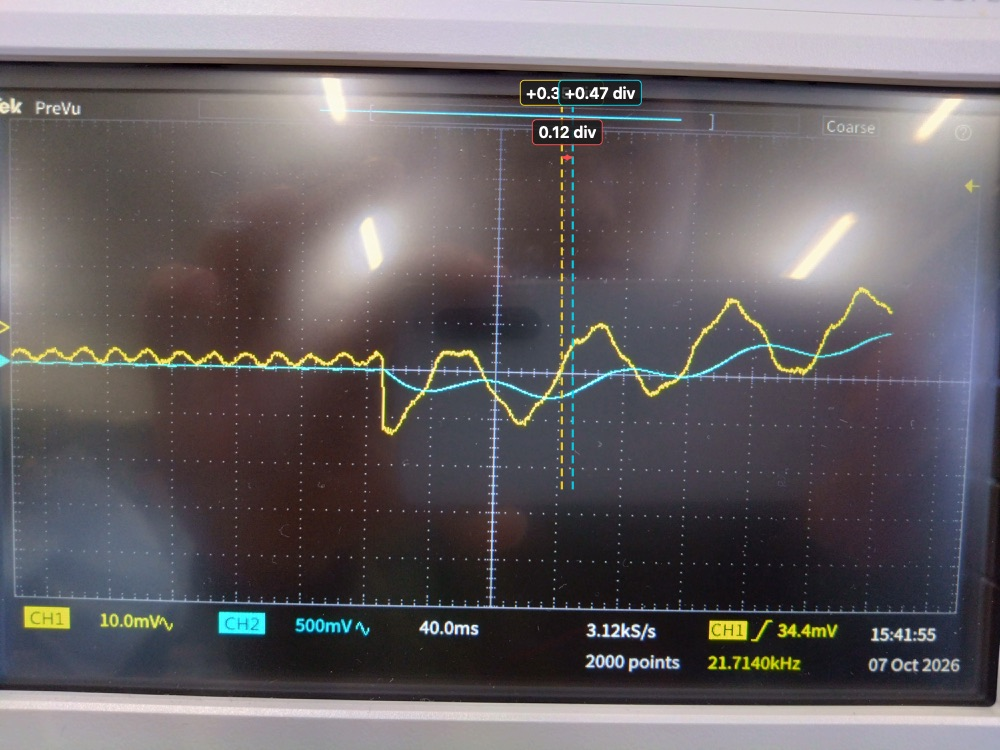
\includegraphics[width=\textwidth,clip]{fig_work_A/赤位相差.jpg}
    \caption{波形2 立ち上がり過渡応答の拡大観測}
    \label{fig:wave2_phase}
  \end{minipage}
  \hfill
  \begin{minipage}[b]{0.48\textwidth}
    \centering
    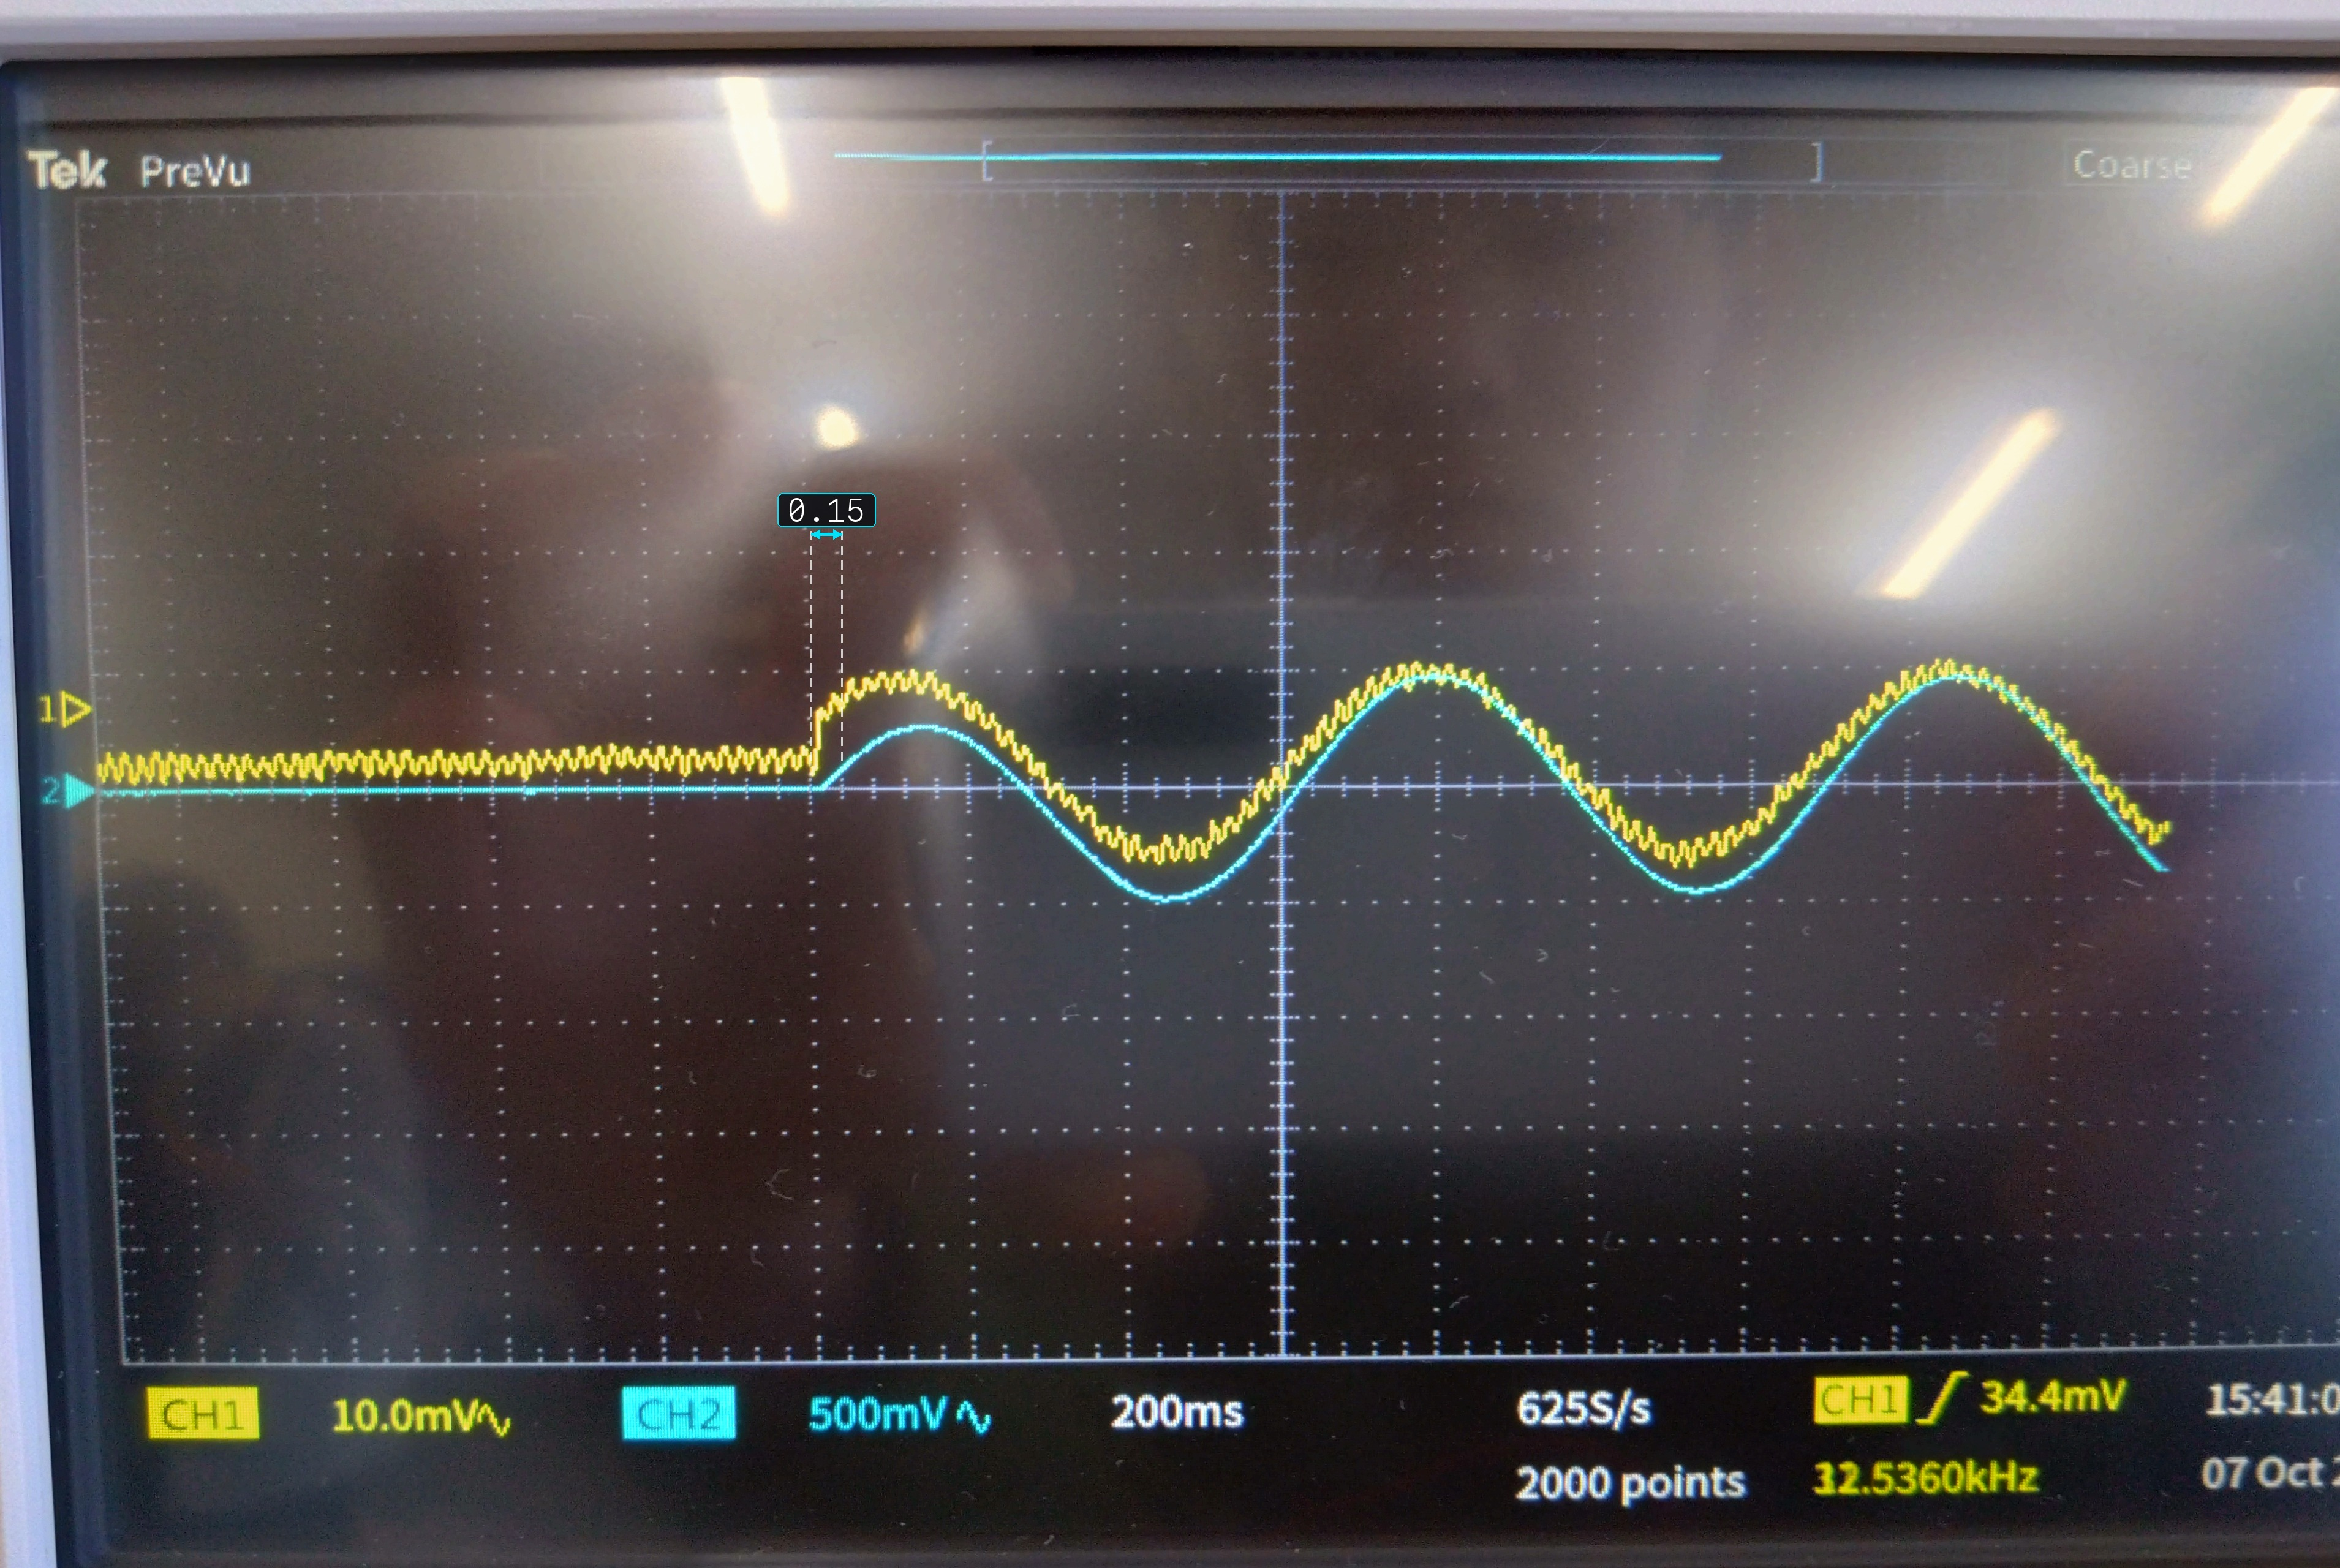
\includegraphics[width=\textwidth,clip]{fig_work_A/青位相差.jpg}
    \caption{波形3 立ち上がり過渡応答の拡大観測}
    \label{fig:wave3_phase}
  \end{minipage}
  \caption{オシロスコープによる高周波成分および立ち上がり過渡応答の拡大観測波形（CH1：$v_i$［黄］，CH2：$v_o$［水色］）}
  \label{fig:waveforms_work_A1_zoom}
\end{figure}


\subsection{ワークA-2：脈拍検出回路による生体脈波の測定結果}

フォトリフレクタ（LBR-127HLD）に被験者の指先を近接させて計測した脈波波形を図\ref{fig:pulse_waveform}に示す．
オシロスコープ画面から直接取得した目盛り読み取り値およびレンジ設定を表\ref{tab:result_raw_work_A2}に示す．
また，これらに基づき算出した周期，周波数，振幅，増幅率，脈拍数，入出力時間差，および位相換算値を表\ref{tab:result_calc_work_A2}に示す．

\begin{figure}[htbp]
  \centering
  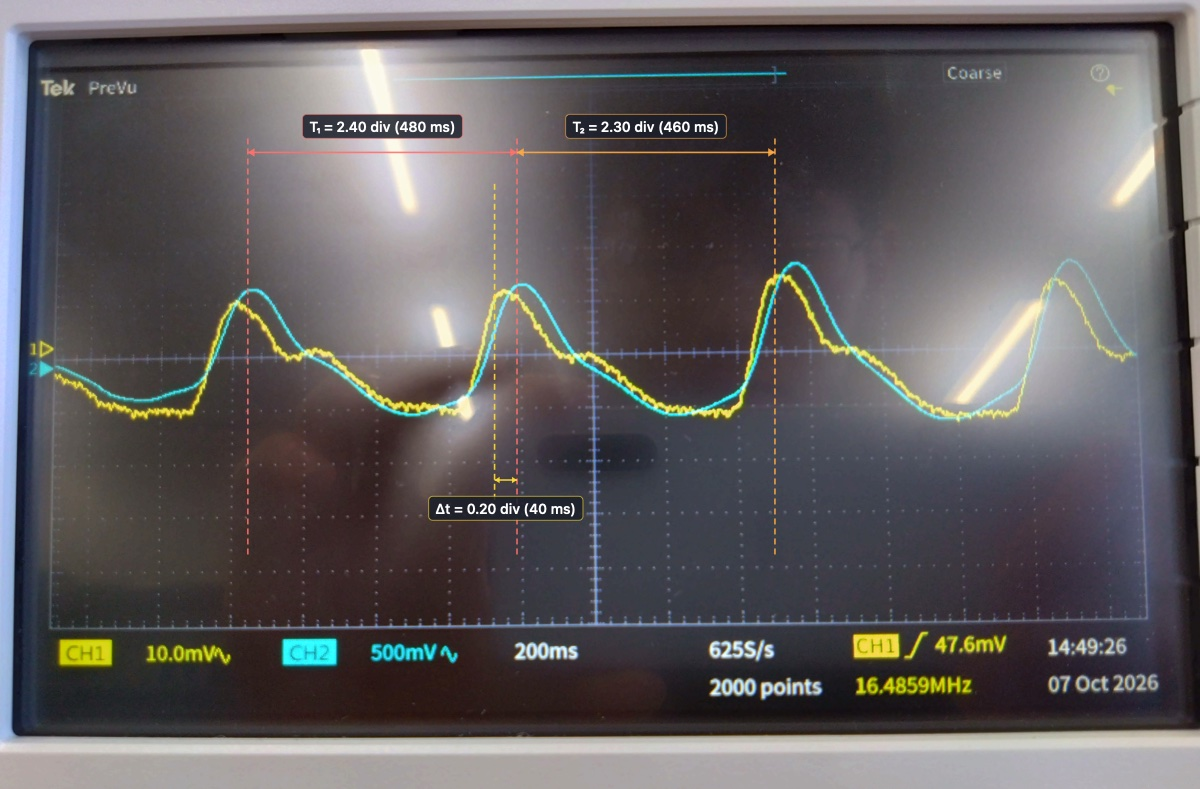
\includegraphics[width=0.75\textwidth,clip]{fig_work_A/脈拍.jpg}
  \caption{オシロスコープに表示された被験者の指先脈波（CH1：$v_i$［黄］，CH2：$v_o$［水色］）}
  \label{fig:pulse_waveform}
\end{figure}

\begin{table}[htbp]
  \caption{生体脈波計測におけるオシロスコープ測定値および設定一覧}
  \centering
  \small
  \begin{tabular}{|l||c|c|}
    \hline
    測定項目                  & 周期の最も長い信号              & 周期が次に長い信号              \\
    \hline\hline
    水平時間軸レンジ（TIME/DIV）    & 200 $\mathrm{ms/div}$  & 200 $\mathrm{ms/div}$  \\
    \hline
    CH1 垂直電圧レンジ（VOLT/DIV） & 10.0 $\mathrm{mV/div}$ & 10.0 $\mathrm{mV/div}$ \\
    \hline
    CH2 垂直電圧レンジ（VOLT/DIV） & 500 $\mathrm{mV/div}$  & 500 $\mathrm{mV/div}$  \\
    \hline
    周期の目盛り読み取り幅           & 3.7 $\mathrm{div}$     & 3.5 $\mathrm{div}$     \\
    \hline
    CH1 ($V_{i,\mathrm{pp}}$) 電圧振幅の目盛り幅 & 2.6 $\mathrm{div}$     & 2.6 $\mathrm{div}$     \\
    \hline
    CH2 ($V_{o,\mathrm{pp}}$) 電圧振幅の目盛り幅 & 2.9 $\mathrm{div}$     & 2.9 $\mathrm{div}$     \\
    \hline
    入出力ピーク間時間差の目盛り幅       & 0.2 $\mathrm{div}$     & 0.2 $\mathrm{div}$     \\
    \hline
  \end{tabular}
  \label{tab:result_raw_work_A2}
\end{table}

\begin{table}[htbp]
  \caption{生体脈波計測における算定諸特性一覧}
  \centering
  \small
  \begin{tabular}{|l||c|c|}
    \hline
    算出項目                   & 周期の最も長い信号 & 周期が次に長い信号 \\
    \hline\hline
    脈波周期 $T$ [ms]          & 740       & 700       \\
    \hline
    脈波周波数 $f$ [Hz]        & 1.35      & 1.43      \\
    \hline
    入力電圧振幅 $V_{i,\mathrm{pp}}$ [mV]      & 26.0      & 26.0      \\
    \hline
    出力電圧振幅 $V_{o,\mathrm{pp}}$ [mV]      & 1450      & 1450      \\
    \hline
    回路増幅率 $V_{o,\mathrm{pp}}/V_{i,\mathrm{pp}}$ [倍]    & 55.8      & 55.8      \\
    \hline
    脈拍数（1分間あたり） [bpm]      & 81.1      & 85.7      \\
    \hline
    入出力時間差 $\Delta t$ [ms] & 40.0      & 40.0      \\
    \hline
    過渡時間差による位相換算値 $\theta$ [rad]   & $-0.340$  & $-0.359$  \\
    \hline
  \end{tabular}
  \label{tab:result_calc_work_A2}
\end{table}


%-----------------------------------------------------------------------------------
\section{考察}

\subsection{波形出力デバイス入力時の増幅率および周波数特性の考察}

表\ref{tab:result_calc_work_A1}に示した波形出力デバイス（ATOM Lite）の測定結果に基づき，設計した二段反転増幅回路の増幅率および周波数選択特性について考察する．

まず，単一低周波信号である波形1（公称1\,Hz正弦波）における増幅率について検討する．
オシロスコープ観測による実測振幅比は $V_{o,\mathrm{pp}}/V_{i,\mathrm{pp}} = 940\,\mathrm{mV} / 20.0\,\mathrm{mV} = 47.0$\,倍であった．
これは，抵抗比に基づく中域公称利得（総合約91.8倍，式(\ref{eq:total_gain})）に対し，約5割強の値である．
この差異の要因について検討する．
第一に，公称91.8倍は理想オペアンプかつ通過帯域中心（$f_L \ll f \ll f_U$）を前提とした中域近似利得である．
実測された周波数 $f \approx 1.52\,\mathrm{Hz}$ は下限遮断周波数 $f_L \approx 0.482\,\mathrm{Hz}$ に比較的近いため，式(\ref{eq:amplitude_transfer})の振幅伝達関数モデルに従えば，
\begin{equation}
  |H(1.52\,\mathrm{Hz})| = 91.8 \cdot \frac{1}{1 + (0.482/1.52)^2} \cdot \frac{1}{1 + (1.52/15.92)^2} \approx 91.8 \cdot 0.908 \cdot 0.991 \approx 82.6\,\text{倍}
\end{equation}
と計算され，低域遮断特性によりすでに公称値から約1割の利得減衰が生じる理論構成となっている．
さらに，抵抗器の公差下限（式(\ref{eq:total_gain_min})より約75.2倍）を考慮してもなお理論利得と実測利得（47.0倍）の間には隔たりが残る．
この要因としては，オペアンプ LM358N の有限な差動開ループ利得および入力インピーダンス，単一電源5\,V駆動に伴う中間バイアス電位のオフセットや動作直線性制約，さらにはブレッドボード配線における接触抵抗や浮遊容量による高域インピーダンス低下などが重畳した複合的影響が考えられる．
なお，ATOM Lite の出力ピンと回路入力端子 $v_i$ の間に直列挿入された保護抵抗（$1\,\mathrm{M}\Omega$）は，ATOM Lite の DAC 内部出力から $v_i$ までの信号を減衰させる役割を果たすが，本測定では CH1 プローブを抵抗後段の端子 $v_i$ に直接接続して入力電圧を観測しているため，観測された利得比 $V_{o,\mathrm{pp}}/V_{i,\mathrm{pp}}$ そのものを低下させる直接要因ではない．

次に，各信号の周波数同定およびフィルタリング特性について検討する．
表\ref{tab:result_calc_work_A1}に示す通り，ATOM Lite の公称周波数設定に対し，オシロスコープ目盛りから算出した実測周波数は低周波成分で約1.43〜1.52\,Hz，高周波成分で約12.5\,Hz（波形2および波形3）となった．
公称値（1\,Hz，100\,Hz，7\,Hz）と実測周波数の間に生じている差異については，合成波における局所的な山・谷の間隔読み取りによる誤差，オシロスコープの時間軸分解能，あるいは ATOM Lite 内部の DAC 出力タイマーや波形テーブル生成周期の設定誤差などの要因が考えられるが，本実験の測定系のみではその主因を特定するには至らないため，公称値と実測値は区別して扱う必要がある．

高周波成分に対する応答に着目すると，波形2（公称1\,Hz $+$ 100\,Hz合成波）の高周波拡大観測（図\ref{fig:waveforms_work_A1_zoom}(a)）において，入力 $v_i$ に重畳していた高周波成分（振幅 18.0\,mV）に対し，出力 $v_o$ では振幅が 500\,mV に抑制されていた．
仮に通過帯域内の中域利得（約92倍）で増幅された場合，出力振幅は約 1650\,mV に達する計算となるため，高域側において明らかな利得低下が生じていることが確認できる．
上限遮断周波数 $f_U \approx 16\,\mathrm{Hz}$（$-40\,\mathrm{dB/dec}$）の2次ローパスフィルタ特性の理論予測に基づけば，高周波ノイズ（商用電源ノイズ50/60\,Hzや照明ノイズ等）に対する減衰効果が期待されるが，本実験で実証されたのは試験波形における振幅抑制傾向であり，商用電源ノイズ等の完全な除去特性については別途定量的な周波数掃引測定による検証が求められる．
また，波形3（公称1\,Hz $+$ 7\,Hz合成波）では高周波成分の出力振幅が 200\,mV として観測された．
なお，波形2・3・4における低周波振幅比（28.6〜51.2倍）は，単一正弦波の線形利得ではなく複数成分が重畳した合成波全体のピーク間振幅比（包絡線比）であるため，周波数成分ごとの真の利得とは区別して解釈する必要がある．


\subsection{生体脈波の周期および脈拍数に関する考察}

被験者の指先を用いてフォトリフレクタ（LBR-127HLD）により検出した生体脈波波形（図\ref{fig:pulse_waveform}，表\ref{tab:result_raw_work_A2}，表\ref{tab:result_calc_work_A2}）について考察する．

測定された指先脈波において，最も長い周期は $T_1 = 740\,\mathrm{ms}$（周波数 1.35\,Hz），次に長い周期は $T_2 = 700\,\mathrm{ms}$（周波数 1.43\,Hz）であり，これらから算出した1分間あたりの脈拍数はそれぞれ 81.1\,bpm および 85.7\,bpm であった．
健常成人の安静時脈拍数は一般に $60 \sim 100\,\mathrm{bpm}$（心拍周期 $600 \sim 1000\,\mathrm{ms}$）の範囲とされることが多い．
本測定で得られた 81.1〜85.7\,bpm はこの安静時生理的範囲に合致しており，本回路系により指先血流変動から生体脈波の周期を抽出し，脈拍数を算定可能であることが確認された．
ただし，本実験では医療用脈拍計等の独立した基準計器との同時測定を行っていないため，得られた脈拍数の測定精度そのものを評価・保証するものではない．

また，最長周期（740\,ms）と次長周期（700\,ms）の間に観測された 40\,ms の周期差については，呼吸運動に伴う自律神経活動の周期変動（呼吸性洞性不整脈など）の可能性が一因として推測されるものの，呼吸状態のモニタリングや長時間の連続心拍記録を実施していないため，単一測定区間におけるこの周期差の原因を特定することはできず，自然な心拍ゆらぎの存在を示唆するにとどまる．


\subsection{入出力信号の時間差と位相差の原因に関する考察}

オシロスコープ観測により得られた入力信号 $v_i$（CH1：黄）と出力信号 $v_o$（CH2：水色）の間における時間差および位相差について考察する．

信号立ち上がり時における過渡応答の拡大観測波形（図\ref{fig:waveforms_work_A1_zoom}(c), (d)）において，急峻な信号変化点に着目すると，いずれの波形においても入力信号 $v_i$（CH1：黄）が先行して変化し，出力信号 $v_o$（CH2：水色）が遅れて追従している様子が明瞭に確認できる．
指先脈波計測（ワークA-2）においても，入出力ピーク間に実測時間差 $\Delta t = 40.0\,\mathrm{ms}$ が観測され，式(\ref{eq:phase_calc_result})による形式的な換算値は $\theta = -0.340\,\mathrm{rad}$（最長周期740\,ms時）および $\theta = -0.359\,\mathrm{rad}$（次長周期700\,ms時）となった．

ここで，周波数伝達関数の定常理論位相角と実測過渡時間差による位相換算値との間に生じる符号の不一致について論じる．
式(\ref{eq:phase_transfer})に脈波の基本周波数 $f \approx 1.35\,\mathrm{Hz}$ を代入して求めた定常正弦波理論位相角は，
\begin{equation}
  \phi(1.35\,\mathrm{Hz}) \approx 2 \left( \arctan\frac{0.482}{1.35} - \arctan\frac{1.35}{15.92} \right) \approx 2 (19.6^\circ - 4.9^\circ) \approx +29.4^\circ \approx +0.513\,\mathrm{rad}
\end{equation}
となり，正の位相進みを示す．
この定常理論モデルが進み位相となる理由は，低周波域（$f = 1.35\,\mathrm{Hz}$）において入力結合コンデンサ等による1次HPFの位相進み（各段約 $+19.6^\circ$）が，帰還コンデンサ等による1次LPFの位相遅れ（各段約 $-4.9^\circ$）を上回るためである．
これに対し，オシロスコープで実測された時間差から算出した値が負の遅れ（$\theta < 0\,\mathrm{rad}$）を示しているのは，以下の物理的・測定論的要因によるものと解釈される：
\begin{enumerate}
  \item \textbf{定常位相特性と過渡時間応答の相違}：
        式(\ref{eq:phase_transfer})の理論位相角 $\phi(f)$ は，同一周波数の定常正弦波が無限時間継続した平衡状態における入出力正弦波のゼロクロス位相関係を規定するものである．
        一方，実験で観測した時間差 $\Delta t$ は，信号の立ち上がり過渡エッジ，あるいは非正弦波である生体脈波のピーク到達時間差を測定した時間領域の応答である．過渡期においては，各増幅段の帰還RC時定数（$R_2 C_2 = 10.0\,\mathrm{ms}$，$R_1 C_1 = 10.0\,\mathrm{ms}$）に伴うコンデンサ充電時間，およびオペアンプ LM358N の有限なスルーレートや内部位相補償容量による応答遅延が直接的な時間遅れとして支配的に現れる．
  \item \textbf{周期換算式の適用限界}：
        式(\ref{eq:phase_calc_result})（$\theta = -2\pi \Delta t / T$）は単一周波数の定常波においてピークまたはゼロクロス間時間差を位相角に変換する定義式であり，過渡応答エッジの時間遅延や高調波を含む複合生体波形のピーク遅れを直接定常周波数位相と同一視することには測定原理上の限界がある．
  \item \textbf{群遅延モデルの周波数依存性}：
        式(\ref{eq:group_delay_transfer})の全回路群遅延式において，$f = 1.35\,\mathrm{Hz}$ における理論群遅延は約 $84.2\,\mathrm{ms}$ と算出され，低周波域ではHPFの進み位相勾配が群遅延に大きく影響する．LPF部のみの時定数の和（約20.0\,ms）は高周波側の遅延特性を近似したものに過ぎず，非正弦波脈波の複雑なスペクトル成分に対するピーク遅延を単一の群遅延数値で完全に説明することは困難である．
\end{enumerate}
したがって，定常伝達関数上の「位相進み特性」と時間領域で観測される「過渡的・応答的な時間遅延」は物理的に異なる現象を捉えたものであり，アナログフィルタの特性評価においては周波数領域と時間領域の挙動を明確に分離して考察する必要がある．


\section{おわりに}
%% ワークAを通じて得られた知見や考察，目的の達成度などについて記述し，ワー
%% クAを総括する．単なる感想ではなく，客観的な総括を行うように注意する．

本実習（ワークA）では，光電容積脈波計測法に基づく脈拍検出回路およびオペアンプを用いたバンドパスフィルタ付き二段反転増幅回路の設計・実装・動作検証を行った．
生体信号特有の微弱性およびノイズ重畳という課題に対し，赤外LEDとフォトトランジスタで構成されるフォトリフレクタ（LBR-127HLD）のバイアス抵抗を選定し，後段に低域遮断周波数 $f_L \approx 0.48\,\mathrm{Hz}$，高域遮断周波数 $f_U \approx 16\,\mathrm{Hz}$，中域理論利得約91.8倍の二段反転増幅回路を構成した．

波形出力デバイス（ATOM Lite）を用いた評価（ワークA-1）では，単一正弦波（波形1）において約47.0倍の実測増幅率が得られ，公称中域利得からの低下について低域遮断特性や回路素子の非理想的要因を踏まえて考察した．また，高周波重畳信号において高域側での振幅抑制傾向を確認し，帯域制限フィルタとしての動作特性を検証した．さらに，時間領域での立ち上がり過渡波形観測を通じて，出力信号の追従応答時間に関する知見を得た．
続いて実施した指先脈波計測実験（ワークA-2）では，被験者の指先血流変動に伴う脈波波形を抽出し，周期（740\,msおよび700\,ms）から安静時心拍数として妥当な脈拍数（81.1\,bpmおよび85.7\,bpm）および周波数（1.35\,Hzおよび1.43\,Hz）を算定できることを確認した．

以上の実験を通じて，アナログフィルタ・増幅回路の設計理論と実機動作における諸特性を多角的に把握し，生体信号検出系におけるアナログ前処理回路の役割と動作特性に関する理解を深めることができた．
